% !TEX TS-program = pdflatex
% !TEX encoding = UTF-8 Unicode

% This is a simple template for a LaTeX document using the "article" class.
% See "book", "report", "letter" for other types of document.

\documentclass[11pt]{exam} % use larger type; default would be 10pt

\usepackage[utf8]{inputenc} % set input encoding (not needed with XeLaTeX)

%%% Examples of Article customizations
% These packages are optional, depending whether you want the features they provide.
% See the LaTeX Companion or other references for full information.

%%% PAGE DIMENSIONS
\usepackage{geometry} % to change the page dimensions
\geometry{a4paper} % or letterpaper (US) or a5paper or....
\geometry{margin=1in} % for example, change the margins to 2 inches all round
% \geometry{landscape} % set up the page for landscape
%   read geometry.pdf for detailed page layout information

\usepackage{graphicx} % support the \includegraphics command and options

\usepackage[parfill]{parskip} % Activate to begin paragraphs with an empty line rather than an indent

%%% PACKAGES
\usepackage{booktabs} % for much better looking tables
\usepackage{array} % for better arrays (eg matrices) in maths
\usepackage{paralist} % very flexible & customisable lists (eg. enumerate/itemize, etc.)
\usepackage{verbatim} % adds environment for commenting out blocks of text & for better verbatim
\usepackage{subfig} % make it possible to include more than one captioned figure/table in a single float
% These packages are all incorporated in the memoir class to one degree or another...

\usepackage{hyperref}
\usepackage{listings}
\usepackage{xcolor}
\usepackage{color}

\usepackage{xhfill}
\usepackage{amssymb}
\usepackage{textcomp}

\usepackage{minted}
\usepackage[T1]{fontenc}
\usepackage{lmodern}

%%% SECTION TITLE APPEARANCE
\usepackage{sectsty}
\allsectionsfont{\sffamily\mdseries\upshape} % (See the fntguide.pdf for font help)
% (This matches ConTeXt defaults)

%%% ToC (table of contents) APPEARANCE
\usepackage[nottoc,notlof,notlot]{tocbibind} % Put the bibliography in the ToC
\usepackage[titles,subfigure]{tocloft} % Alter the style of the Table of Contents
\renewcommand{\cftsecfont}{\rmfamily\mdseries\upshape}
\renewcommand{\cftsecpagefont}{\rmfamily\mdseries\upshape} % No bold!

%%% END Article customizations

%%% The "real" document content comes below...
\title{Übungsaufgaben EIDI 2 \\ \small \color{magenta}Version 1.1.2}
\author{Christian Femers}
%\date{} % Activate to display a given date or no date (if empty),
         % otherwise the current date is printed 


\newcommand{\code}[1]{\mintinline{Java}|#1|}
\newcommand{\fillinline}[1]{\ifprintanswers\fillin[\code{#1}][3cm]\fi\xrfill[-1pt]{0.2mm}}
\newcommand{\fillinlinexl}[1]{\ifprintanswers\fillin[\code{#1}][9cm]\fi\xrfill[-1pt]{0.2mm}}

\renewcommand{\solutiontitle}{\noindent\textbf{Lösung:}\enspace}

\setminted{
    linenos=true,
    frame=single,
    tabsize=4,
}

\usepackage[german]{babel}
\usepackage{csquotes}

\pointsinrightmargin
\bracketedpoints
\pointpoints{Pinguin}{Pinguine}
\checkboxchar{$\square$}
\checkedchar{$\blacksquare$}

\begin{document}
\maketitle

%\printanswers % ANSWERS

\ifprintanswers
\begin{framed}{\vspace{8.5cm}\begin{center}\color{red}\textbf{ACHTUNG: LÖSUNGEN}\end{center}\vspace{8.75cm}}\end{framed}
\newpage
\fi

\begin{questions}
\question Was sind \textbf{keine} Java-Schlüsselwörter?
\begin{checkboxes}
\choice \texttt{final}
\choice \texttt{const}
\CorrectChoice \texttt{var}
\choice \texttt{short}
\CorrectChoice \texttt{false}
\choice \texttt{case}
\choice \texttt{class}
\CorrectChoice \texttt{main}
\choice \texttt{static}
\choice \texttt{throw}
\choice \texttt{throws}
\CorrectChoice \texttt{null}
\end{checkboxes}
\filbreak
\question Zu was evaluieren die folgenden Java-Ausdrücke? 
\begin{parts}
\part \code{3 - 0}:\fillinline{3}
\part \code{-7 / 2}: \fillinline{-3}
\part \code{-7 / 2.0}: \fillinline{-3.5}
\part \code{-7d / 2}: \fillinline{-3.5}
\part \code{true ? 3 : 2 + 1}: \fillinline{3}
\part \code{0.25 * 8}: \fillinline{2.0}
\part \code{42 * 2 + "Niugnip" + 42 + 2}: \fillinline{84Niugnip422}
\part \code{(long) 1.0 + "java" + 1}: \fillinline{1java1}
\part \code{4 + ~-1 >= 5 ? 2 * 0 : 3 / 2 + 2}: \fillinline{3}
\part \code{'a' + 25 - 'z'}: \fillinline{0}
\part \code{(8745 / 61) + (83 / 0)}: \fillinlinexl{java.lang.ArithmeticException: / by zero}
\part \code{0 / 1 == 0 ? null : "hallo"}: \fillinline{null}
\part \code{(byte) 127 + 1}: \fillinline{128}
\end{parts}
\filbreak
\question Betrachten Sie den folgenden Code-Auszug:
\begin{minted}{Java}
Integer input = getUserInput();

if (input == (Integer) 42)
	System.out.println("Antwort gefunden");
else
	System.out.println("Weitersuchen");
	
if ("83".equals("" + (int) input))
	System.out.println("83 gefunden");
\end{minted}
Welche der folgenden Aussagen treffen zu? Nehmen Sie an, dass der Code kompiliert und betrachten sie ihn als Algorithmus. Gehen Sie nur von dem aus, was sie sehen können. 
\begin{checkboxes}
\choice In Zeile 3 wird der Wert von \texttt{input} mit \texttt{42} verglichen.
\CorrectChoice In Zeile 3 werden Objekte auf Referenzgleichheit geprüft
\CorrectChoice \texttt{Antwort gefunden} wird möglicherweise für eine Eingabe von \texttt{42} ausgegeben.
\choice Für die Eingabe 42 wird nie \texttt{Antwort gefunden} ausgegeben werden.
\CorrectChoice Möglicherweise wird \texttt{Weitersuchen} für eine Eingabe von \texttt{42} ausgegeben.
\choice Möglicherweise wird \texttt{Antwort gefunden} und \texttt{Weitersuchen} für eine Eingabe von \texttt{42} ausgegeben.
\CorrectChoice Bei der Eingabe von \texttt{83} wird immer \texttt{Weitersuchen} und \texttt{83 gefunden} ausgegeben.
\choice \texttt{83 gefunden} wird nie ausgegeben werden.
\choice In Zeile 8 wird auf Referenzgleichheit geprüft.
\CorrectChoice In Zeile 8 werden zwei Strings zeichenweise miteinander verglichen.
\choice Für die Eingabe -83 wird \texttt{83 gefunden} ausgegeben.
\CorrectChoice Bei Zeile 3 wird nie eine \texttt{NullPointerException} geworfen werden.
\CorrectChoice Zeile 8 wirft möglicherweise eine \texttt{NullPointerException}.
\choice Bei Zeile 8 wirft \texttt{equals} eine \texttt{IllegalArgumentException}.
\choice Die Ausgabe ist nicht deterministisch.
\CorrectChoice Möglicherweise wird gar nichts in die Konsole ausgegeben.
\end{checkboxes}
\question Zu welchem Wert evaluieren die folgenden Ausdrücke, vorausgesetzt die \code{int}-Variable \texttt{x} hat vor jeder Teilaufgabe den Wert 0?
\begin{parts}
\part \code{x++}: \fillinline{0}
\part \code{x = x = x++}: \fillinline{0}
\part \code{x++ + ++x}: \fillinline{2}
\part \code{--x != ++x}: \fillinline{true}
\part \code{--x - --x - x}: \fillinline{3}
\part \code{x++ == x++ ? x-- - 1 : --x + 1}: \fillinline{2}
\part \code{x++ * x++ * x++}: \fillinline{0}
\end{parts}
\filbreak
\question Was sind erlaubte Bezeichner für Variablen in Java (ab Version 9)?
\begin{checkboxes}
\choice \texttt{ein name}
\choice \texttt{const}
\CorrectChoice \texttt{var}
\CorrectChoice \texttt{µPC}
\CorrectChoice \texttt{\$name}
\choice \texttt{\_}
\CorrectChoice \texttt{\_\_}
\choice \texttt{public}
\CorrectChoice \texttt{CLASS}
\choice \texttt{42sinn}
\CorrectChoice \texttt{main}
\CorrectChoice \texttt{\_mäin\_}
\choice \texttt{pingu!n}
\choice \texttt{null}
\end{checkboxes}
\filbreak
\question Erstellen sie das Kontrollflussdiagramm zu folgendem Java-Code-Auszug. Die Methode \code{read()} gibt dabei einen \code{int} zurück, \code{write(int)} gibt den übergebenen \code{int}-Wert auf der Konsole aus.
\begin{minted}{Java}
final int a = read();
int b = a;
OUTER: for(int i = 0; i < 5; i++) {
	switch(b) {
		case 1:
		case 2: b++; continue;
		case 5:
		case 4: b--; break;
		case 3: break OUTER;
	}
	write(b);
}
write(b);
\end{minted}
\begin{solution}\par\nobreak
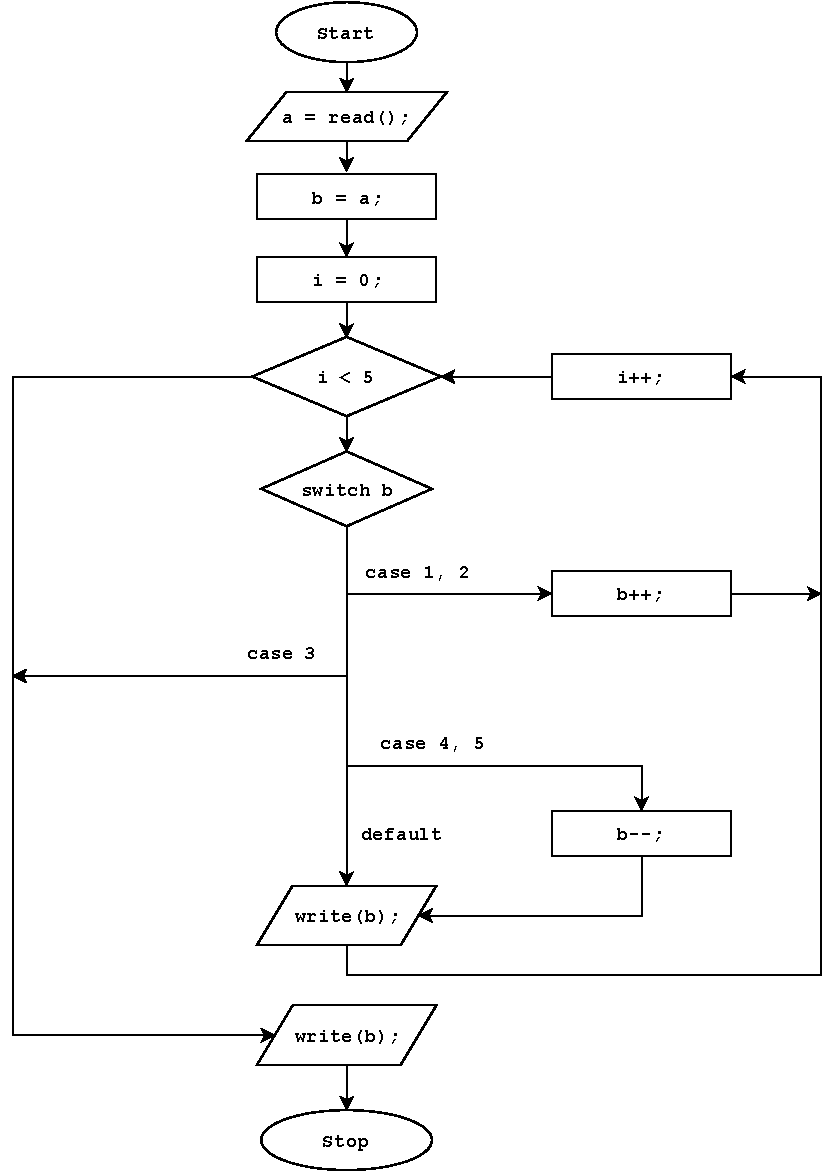
\includegraphics[width=\linewidth]{kontrollfluss.pdf}\par
Es gibt verschiedene richtige Wege, \code{switch} darzustellen. Je nachdem ist es sicherer, die \code{case 1, 2} aufzuspalten in zwei Pfeile \code{case 1} und \code{case 2}. Es müsste jedoch beides als richtig angesehen und gewertet werden.
\end{solution}

\end{questions}

\end{document}